\documentclass{beamer}

\usetheme{clearmatics} 

\progressbar  % Comment this out to remove the progress bar from the foot line

\usepackage[english]{babel}
\usepackage{amsmath}
\usepackage{mathtools}
\usepackage{lipsum}

\usepackage{tikz}
\usetikzlibrary{shapes,arrows}
\usepackage{pgfplots}
\usepackage{fancybox}

\title{\large Fiat and Crypo Currencies}
\subtitle{\small Invesco Seminar, Cambridge University} 
\date{\small 19 May 2017}
\author{\small Robert Sams} % Presenter name for the title page

\address{30 Great Guildford Street\newline London SE1 0HS} % Clearmatics address for the final slide
\contact{Robert Sams} 
\position{Chief Executive Officer} 
\email{rs@clearmatics.com}
\phone{+44 20 3654 4875} 

\usecolortheme{clearmatics}

%%%%%%%%%%%%%%%%%%%%%%%%%%%%%%%%%%%%%%%%%%%%%%%%%%%%%%%%%%%%%%%%%%%%%%%%%%%%
\begin{document}

\begin{frame}
  \titlepage
\end{frame}


\begin{frame}
  \frametitle{Fiat and Crypto Currency}

  \begin{block}{Fiat Currency}
    \begin{itemize}
    \item A form of money that is neither \textbf{redeemable into} nor \textbf{backed by
        another asset}. 
    \item Issued by a \textbf{central bank}.
    \end{itemize}
  \end{block}
  
  \begin{block}{Crypto Currency}
    \begin{itemize}
    \item A form of money that is neither \textbf{redeemable into} nor \textbf{backed by
        another asset}.
    \item Issued by a \textbf{protocol}.
    \end{itemize}
  \end{block}

  \pause
  
  \begin{center}
    {\Large Main difference? Rules-vs-discretion}
  \end{center}
  
\end{frame}

\begin{frame}
  \frametitle{Three functions of money}

  \begin{itemize}
  \item Medium-of-Exchange
  \item Store-of-Value
  \item \textbf{Unit-of-Account}
  \end{itemize}

  \begin{block}{}
    Cryptocurrency performs two of the three functions. Whether it
    does so well or badly depends on one's perspective.
  \end{block}
  
\end{frame}

\begin{frame}{Bitcoin Volatility}
  \begin{center}
    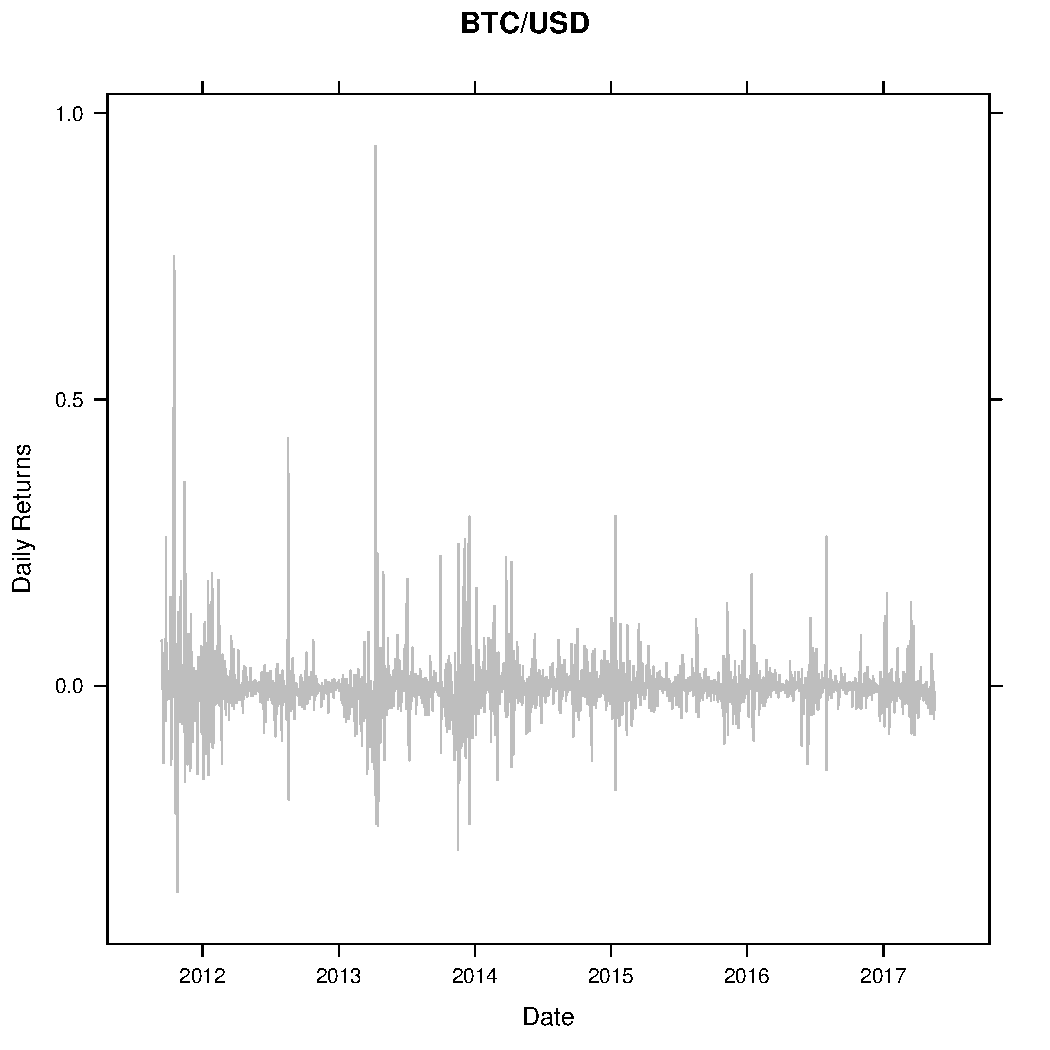
\includegraphics[keepaspectratio,width=0.75\textwidth]{btcror.pdf} 
  \end{center}
\end{frame}

\begin{frame}{Do you see a trend?}
  \begin{center}
    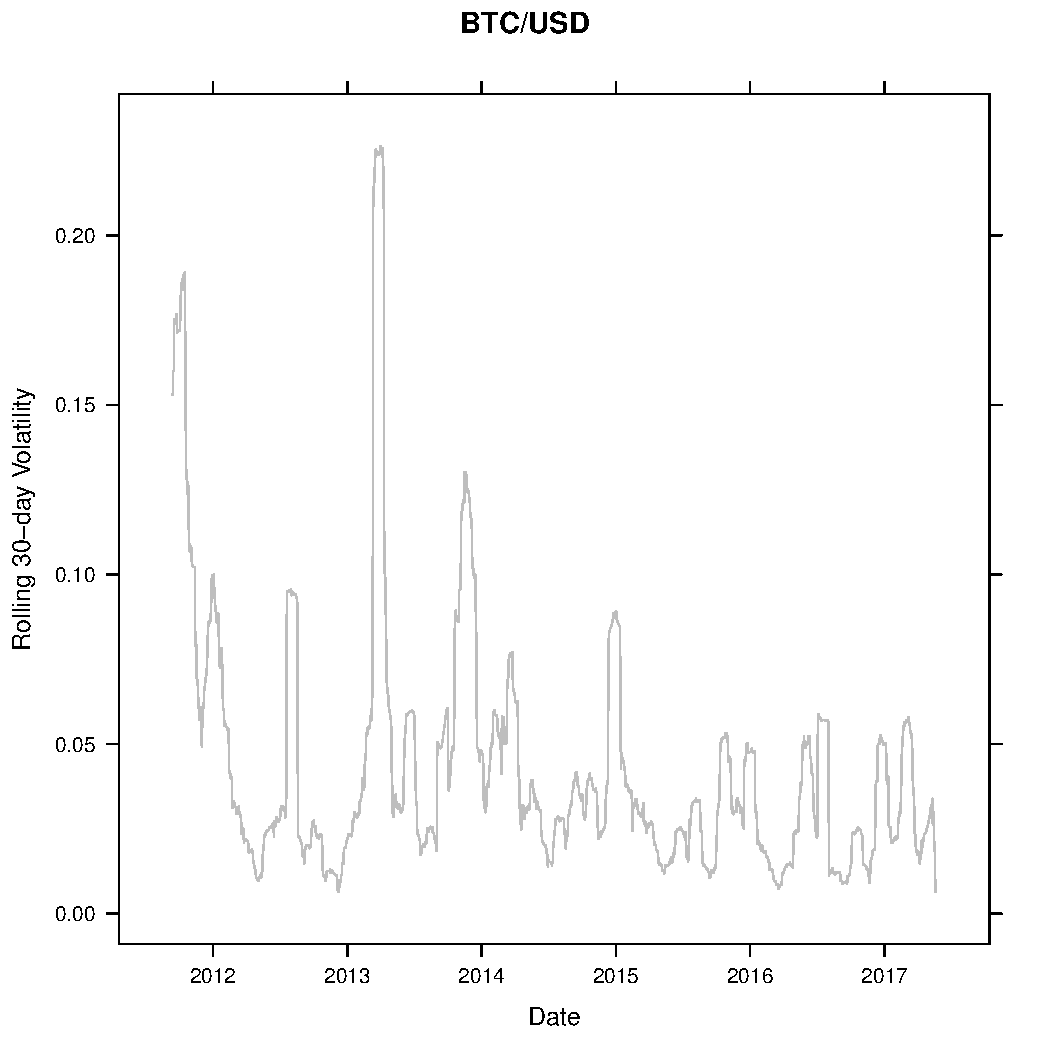
\includegraphics[keepaspectratio,width=0.75\textwidth]{btcvol.pdf} 
  \end{center}
\end{frame}

\begin{frame}
  \frametitle{Will Bitcoin Volatility Decline?}

  \begin{description}
  \item[Short answer] No.
  \item[Longer answer] No, unless future demand becomes more
    predictable.
  \end{description}
  
  And, no, a more liquid BTC market will not make Bitcoin's
  price more stable\dots

  \begin{block}{}
    \emph{The main volatility in bitcoin comes from variability in
    speculation, which in turn is due to the genuine uncertainty about
    its future. More efficient liquidity mechanisms don't help
    reduce genuine uncertainty.}\\\textbf{Nick Szabo}
  \end{block}
  
\end{frame}

\begin{frame}
  \frametitle{Deterministic Coin Supply}

  \begin{block}{What is ``deterministic coin supply''?}
    The growth rate of coin supply is completely specified in advance
    and is not influenced by facts outside of the system.
  \end{block}

  \begin{itemize}
  \item This is \emph{not} "digital gold"
  \item Even gold has a supply that responds to its price
  \item Bitcoin is more like a "digital collectable"
  \end{itemize}

\end{frame}

\begin{frame}
  \frametitle{Coin Demand}
  \begin{description}
  \item[Transactional Coin Demand $CD_{T}$] Desire to hold a certain
    quantity of coins for the purpose of making transactions.
  \item[Speculative Coin Demand $CD_{S}$] Desire to hold a certain
    quantitiy of coins to speculate on future increases in coin
    price / purchasing power. 
  \end{description}

  \begin{block}{Coin demand made up of both transactional and
      speculative motives}
    \begin{equation*}
      CD = CD_{T} + CD_{S}  
    \end{equation*}
  \end{block}
\end{frame}

\begin{frame}
  \frametitle{Coin Demand}
  \begin{block}{Coin demand is a quantity of \textbf{purchasing power}}
    \begin{equation*}
      CD = P \times Q
    \end{equation*}
    \begin{description}
    \item[$P$] purchasing power, coin price of a broad basket of goods
      and services
    \item[$Q$] quantity of coins demanded given $P$
    \end{description}
  \end{block}
\end{frame}

\begin{frame}
  \frametitle{Coin Demand Curve (and fixed supply)}
  \begin{columns}
    \column{0.6\linewidth}
    \begin{block}{$CD$ Change with Fixed Supply}
      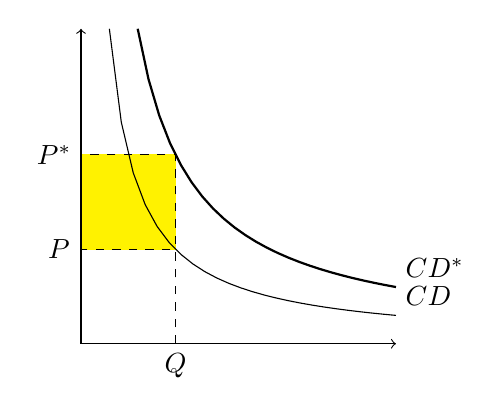
\begin{tikzpicture}[scale=0.40]
        \draw[fill=yellow,yellow] (3,3) rectangle (0,6); % yellow box
        \draw[<->] (0,10) -- (0,0) -- (10,0); % axis
        \draw[domain=0.9:10] plot (\x, {9/\x}); % CD curve
        \node[above right] at (10,0.9) {$CD$};
        \draw[thick,domain=1.8:10] plot (\x, {18/\x}); % CD* curve
        \node[above right] at (10,1.8) {$CD^{*}$};
        \draw[dashed] (3,0) -- (3,3) -- (0,3) node[left]{$P^{}$}; % marks
        \draw[dashed] (3,0) node[below]{$Q$} -- (3,6) -- 
        (0,6) node[left]{$P^{*}$};
      \end{tikzpicture}
    \end{block}
    \column{0.4\linewidth} 
    With a deterministic supply protocol like Bitcoin's, an X\%
    increase in \textbf{demand} ($CD$ to $CD^{*}$) causes an X\%
    increase in \textbf{coin price} ($P$ to $P^{*}$) because supply is
    fixed in the period.
  \end{columns}
\end{frame}

\begin{frame}
  \frametitle{Coin Demand Curve (fully elastic supply)}
  \begin{columns}
    \column{0.6\linewidth}
      \begin{block}{$CD$ Change with Elastic Supply}
        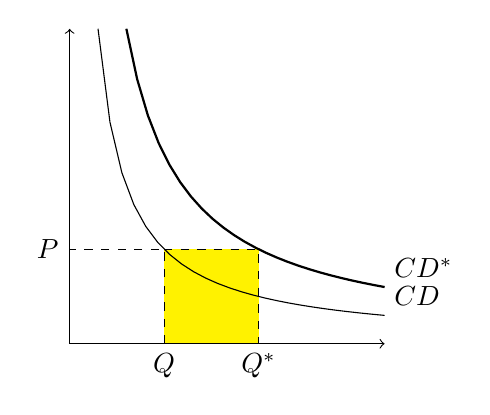
\begin{tikzpicture}[scale=0.40]
          \draw[fill=yellow,yellow] (3,3) rectangle (6,0); % yellow box
          \draw[<->] (0,10) -- (0,0) -- (10,0); % axis
          \draw[domain=0.9:10] plot (\x, {9/\x}); % CD curve
          \node[above right] at (10,0.9) {$CD$};
          \draw[thick,domain=1.8:10] plot (\x, {18/\x}); % CD* curve
          \node[above right] at (10,1.8) {$CD^{*}$};
          \draw[dashed] (3,0) node[below]{$Q$} -- (3,3) -- 
          (0,3) node[left]{$P^{}$}; % marks
          \draw[dashed] (3,3) -- (6,3) -- 
          (6,0) node[below]{$Q^{*}$};
        \end{tikzpicture}
      \end{block}
    \column{0.4\linewidth} 
    An X\% increase in \textbf{demand} ($CD$ to $CD^{*}$) causes an
    X\% increase in \textbf{coin quantity} ($Q$ to $Q^{*}$) because
    supply can change in the period.
  \end{columns}
\end{frame}

\begin{frame}
  \frametitle{Deterministic Supply Causes Volatility}
  \begin{itemize}
  \item If demand growth exceeds pre-programmed supply
    growth, coin price will increase.
  \item But if we \textbf{expect today} that this will happen in
    future, then price increase will happen today (\textbf{``Law of
      Iterated Expectations''}).
  \item Therefore, bitcoin price reflects today's expectations of
    future demand growth.
  \item \dots and deterministic supply \textbf{creates speculative
      demand} $CD_{S}$.
  \end{itemize}

  \begin{block}{A prediction market on itself}
    So bitcoin price is a like a prediction market on the growth rate
    of its own future adoption. Price volatility reflects irreducible
    uncertainty about its future. 
  \end{block}
\end{frame}

\begin{frame}
  \frametitle{``So it's like a growth stock, right?''}

  \begin{block}{}
    Transactional coin demand $CD_{T}$ is inversely related to coin
    volatility.
  \end{block}

  The more volatile the coin, the less useful it is as a medium of
  exchange.

  \begin{itemize}
  \item Volatility raises \textbf{transaction costs} for merchants.
  \item Volatility renders coin useless as a \textbf{unit-of-account}.
  \item Volatility increases need for \textbf{re-balancing}.
  \end{itemize}

  \begin{block}{No, it's not like a growth stock}
    The stock price of a young, high growth company is also
    volatile. But the volatility of the a growth company's stock
    \textbf{does \emph{not} influence the demand for its product}. But
    the volatility of bitcoin \emph{does} influence the demand for
    bitcoin as a medium-of-exchange.
  \end{block}
\end{frame}

\begin{frame}
  \frametitle{Elastic Coin Supply}
  \begin{block}{\textbf{Stablecoin}}
    At the end of some pre-defined interval of time (the \emph{rebase
      period}, every $n$ blocks), if the change in coin price of the
    interval is X\%, change coin supply by X\%.
    \begin{eqnarray*}
      Q_{i} &=& Q_{i-1} \times \frac{P_{i}}{P_{i-1}}\\
      \Delta_{i} &=& Q_{i} - Q_{i-1}
    \end{eqnarray*}
    , where $i$ is the i-th rebase period, $Q$ is coin supply and $P$
    is coin price.
  \end{block}
\end{frame}

\begin{frame}
  \frametitle{Theoretical Lineage}

  \begin{block}{Bitcoin}
    \begin{itemize}
    \item Gold standard
    \item Austrian Economics  
    \end{itemize}
  \end{block}

  \begin{block}{Stablecoin}
    \begin{itemize}
    \item Milton Friedman's ``k-percent rule''
    \item Irving Fisher's ``Dollar Stabilisation''
    \end{itemize}
  \end{block}

  \begin{itemize}
  \item Both favour ``rules over discretion'' w.r.t. money
    supply.
  \item These theories assume fractional reserve banking.
  \item Differing opinions about nature of money demand.
  \item Ironically, Bitcoin gives rise to very ``Keynsian-like'' money
    demand.
  \end{itemize}
  
\end{frame}

\begin{frame}
  \frametitle{Two Hard Problems}
  \begin{enumerate}
  \item \textbf{Coin distribution}. How is $\Delta_{i}$ distributed?
  \item \textbf{Data representation}. How can $P_{i}$ be represented
    inside the network in a way that requires minimal trust?
  \end{enumerate}

  \begin{block}{Solution attempts}
    \begin{itemize}
    \item Robert Sams, \emph{A Note on Cryptocurrency Stabilisation: Seigniorage Shares}\\
      \texttt{https://github.com/rmsams/stablecoins}
    \item Vitalik Buterin, \emph{The Search for a Stable Cryptocurrency}\\
      \texttt{https://blog.ethereum.org/2014/11/11/search-stable-cryptocurrency/}
    \end{itemize}
  \end{block}

\end{frame}


\begin{frame}
  \frametitle{Credit Money}

  \begin{block}{Two Types of Money}
  \begin{tabular}{lll}
    Attribute                 & CBM & CoBM \\\hline
    Who issues it?            & central bank       & comm. bank\tabularnewline
    Who can own it?           & banks, some FMI    & everyone\tabularnewline
    How is it transferred?    & CB RTGS system     & various systems\tabularnewline
    How is it created?        & asset purchases    & bank loans\tabularnewline
    Does it have credit risk? & no                 & yes\tabularnewline
    What does it yield?       & policy rate        & LIBOR +/-\tabularnewline
    % \bottomrule
  \end{tabular}
\end{block}

\end{frame}

\begin{frame}
  \frametitle{Coexistence}
  \begin{block}{}
    Why can't you open an account at the central bank? 
  \end{block}

  \begin{itemize}
  \item CBM accessible only by banks (mostly)
  \item Competition with bank deposits, macro stability risk
  \end{itemize}
  
\end{frame}

\begin{frame}
  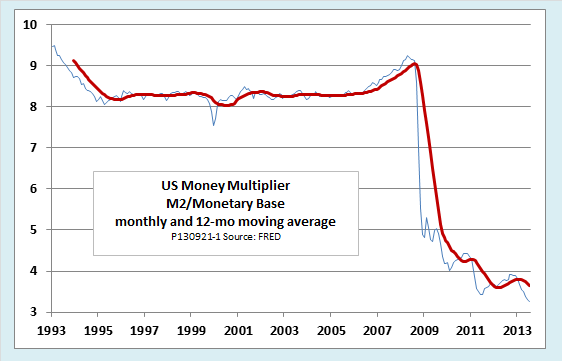
\includegraphics[scale=0.65]{images/money-multiplier.png}
\end{frame}

\begin{frame}
  \frametitle{The Future\dots}

  \large
  
  \begin{itemize}
  \item Central Bank Digital Currency
  \item[] \textbf{OR}
  \item Cryptocurrency (Stablecoin) Base Money
  \end{itemize}
  
\end{frame}

\begin{frame}
  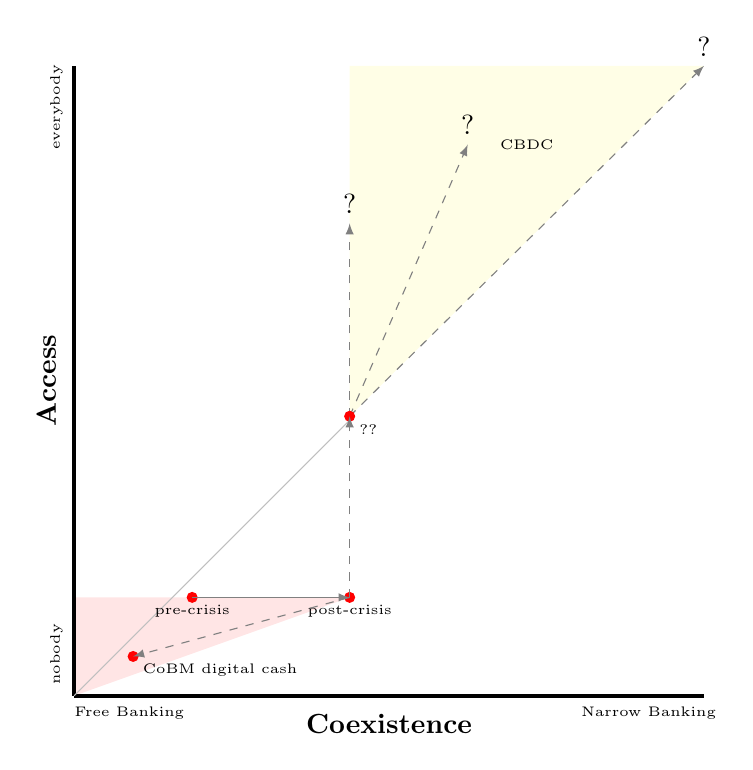
\begin{tikzpicture}

    % cbdc scenario
    \path[fill=yellow!10] (3.5,3.55) -- (3.5,8) -- (8,8);
    \draw[-latex, dashed, draw=black!50] (3.5,3.55) -- (3.5,6) node[above] {?};
    \draw[-latex, dashed, draw=black!50] (3.5,3.55) -- (5,7) node[above] {?};
    \draw[-latex, dashed, draw=black!50] (3.5,3.55) -- (8,8) node[above] {?};
    \node at (5.75,7) {\tiny CBDC};

    % CoBM scenario
    \path[fill=red!10] (0,1.25)--(3.5,1.25)--(0,0);
    \coordinate (comb) at (0.75,0.5);
    \fill[red] (comb) circle (2pt);
    \node[yshift=-5pt, right] at (comb) {\tiny CoBM digital cash};

    % axes
    \draw[ultra thick] (0,0) node[xshift=20pt, below]{\tiny Free
      Banking} -- (8,0) node[xshift=-20pt, below]{\tiny Narrow Banking};
    \draw[ultra thick] (0,0)  node[yshift=15pt, left]{\tiny
      \rotatebox{90}{nobody}} --(0,8) node[yshift=-15pt, left]{\tiny \rotatebox{90}{everybody}};
    \draw[draw=black!25] (0,0) -- (3.55,3.55);

    % axis labels
    \node[yshift=-10pt] at (4,0) {\textbf{Coexistence}};
    \node[xshift=-10pt] at (0,4) {\rotatebox{90}{\textbf{Access}}};

    % pre-crisis
    \coordinate (pre) at (1.5,1.25);
    \fill[red] (pre) circle (2pt);
    \node[yshift=-5pt] at (pre) {\tiny pre-crisis};

    % post-crisis
    \coordinate (post) at (3.5,1.25);
    \fill[red] (post) circle (2pt);
    \node[yshift=-5pt] at (post) {\tiny post-crisis};

    % next
    \coordinate (next) at (3.5,3.55);
    \fill[red] (next) circle (2pt);
    \node[yshift=-5pt, right] at (next) {\tiny ??};

    % edges
    \draw[-latex, draw=black!50] (pre)--(post);
    \draw[-latex, dashed, draw=black!50] (post)--(next);
    \draw[-latex, dashed, draw=black!50] (post)--(comb);

  \end{tikzpicture}
\end{frame}

\end{document}
